\documentclass[dvipsnames,authoryear,11pt]{article}


\usepackage{graphicx}
\usepackage{caption}
\usepackage{subcaption}

\usepackage{setspace}
%\doublespacing

%\usepackage{lineno}
%\linenumbers
%\modulolinenumbers[5]

\usepackage{hyperref}
\usepackage{booktabs}
\usepackage{algorithm,algorithmic}
\usepackage{amsmath}
\usepackage[english]{babel}
\usepackage[latin1]{inputenc}
%\usepackage[utf8]{inputenc}
\RequirePackage{natbib}
\usepackage{multirow}
\usepackage{arydshln}

\allowdisplaybreaks
\usepackage{geometry}
\geometry{a4paper,left=1in,right=1in,top=0.9in,bottom=1.3in}
\usepackage{tikz}
\usetikzlibrary{arrows,snakes,backgrounds}

\newtheorem{definition}{Definition}
\newtheorem{example}{Example}


\usepackage{amssymb}

\usepackage{amssymb}
\newcommand{\nb}[3]{
	{\colorbox{#2}{\bfseries\sffamily\scriptsize\textcolor{white}{#1}}}
	{\textcolor{#2}{\sf\small$\blacktriangleright$\textit{#3}$\blacktriangleleft$}}}
\newcommand{\version}{\emph{\scriptsize$-$Id$-$}}

% COMANDS TO LEAVE COMMENTS
\newcommand{\FL}[1]{\nb{FL}{blue}{#1}}

\newcommand{\refp}[1]{(\ref{#1})}




%opening


\title{The truck-and-freighter routing problem}
\author{ORO - Optimization in Trabnsportation and Logistics \\
	Project at home }
\date{2019}

\begin{document}
	
	\maketitle

%	\begin{abstract}
		
%	\end{abstract}

\section{Project organization}

The goal is to propose a mixed integer linear program to model this problem and to implement it.

\subsection*{Conditions}

\begin{itemize}
	\item The project is to be made by pair/ groups of three. 
	\item Allowed solvers : CBC, Gurobi, CPLEX.
	\item Julia version: must run in 1.2
\end{itemize}


\subsection*{Deliverables}

\begin{itemize}
	\item A report describing your model and experiments. Do not forget to properly comment each notation, constraints and hypothesis.
	\item A source code in Julia.
	\item The project to be handed out on madoc with all your files (code, report, instances, ...). Make sure everything needed to run your code is given.
	\item Date due: to be decided in class, will be written on madoc.
\end{itemize}

\subsection*{Provided material}

\begin{itemize}
	\item The LaTeX source of this document (may be used as a template for your report).
	\item Instances: see the readme file in the instances directory.
	\item Two Julia files: parser.jl and main.jl to parse instances and read your program.
	\item Visualization: a python notebook to run in jupyter to vizualize some results.
\end{itemize}


\section{Problem description}

The truck-and-freighter routing problem consists in delivering goods starting from a principal distribution center to the multiple customers in a city. The specificity of the problem is that the delivery of goods is performed by an innovative type of truck\footnote{\url{http://bil.libner.com}}, where a small electric truck (called city freighter) can travel inside a larger truck (called truck in the following). The city implements an innovative logistics delivery policy and some streets are forbidden to traditional trucks. 
As a result, some customers can be served only by the city freighter. 

In the Truck\&Freighter Routing Problem (TFRP), customers are all delivered from a depot located outside of the city.
To travel to the city center, the large truck leaves this depot, carrying the city freighter. 
Both vehicles can separate and join again at dedicated parking areas. In terms of capacity, the large truck can be considered as having an infinite capacity. The city freighter has a more limited capacity, but it can be resupplied several times by the large truck at parking areas. The day is considered to start at time $0$ and end at the end of the time horizon $T$. All trucks should be back at the depot by this time.

Each customer has a location, a quantity and a time window. All customer should be served before the end of their time window. 
If a truck arrives at a customer before the opening of the time window, it has to wait until this time. 

The routing costs are considered to be equal to the sum of vehicle routing traveling times. 
Note that no cost is accounted for when the small city freighter travels within the large truck. 

The problem consists of designing the routes of the truck and city freighter, including determining when they travel together and separately and where they separate and join, such that all routes start and end at the depot, customers are served within their respective time windows, vehicles capacity are respected, and traveling costs are minimized. 

This problem is illustrated on Figure \ref{fig:fig1}.

\begin{figure}[h]
	\centering
	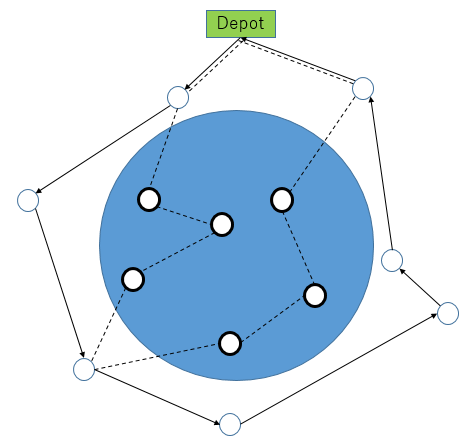
\includegraphics[width=0.6\linewidth]{figure}
	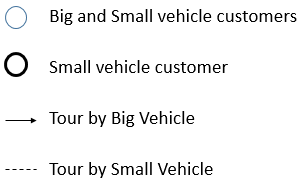
\includegraphics[width=0.3\linewidth]{legende}
	\caption{Typical solution of the truck and freigter routing problem}
	\label{fig:fig1}
\end{figure}

\section{Notation}
	
To model the problem, the following notation is given 
	\subsection{Sets and data}
	Sets: 
	\begin{itemize}
		\item $J=\{1,...,n\}$: set of customers.
		\item vertex $0$ and $n+1$ model the depot.
		\item $J_S \subset J$: nodes which can be served by the small truck only
		\item $P$: set of transfer nodes (parking areas)
		\item $V=\{0;n+1\} \cup J \cup P$
	\end{itemize}

	Data:
	\begin{itemize}
		\item $c_{ij}^B$: cost of going from node $i\in V$ to node $j \in V$ with the big truck
		\item $c_{ij}^S$: cost of going from node $i\in V$ to node $j \in V$ with the small truck alone
		\item $q_j$ demand of customer $j\in J$
		\item $Q$ capacity of the small truck
		\item $t_{ij}$: time of traveling from node $i\in V$ to node $j \in V$
		\item $s_j$: duration of service at customer $j\in J$
		\item $[a_j,b_j]$: customer $j\in J$ time window
		\item $T$ time horizon.
	\end{itemize}

In this project we assume that $c_{ij}^B=t_{ij}$.
For the city freighter, a ratio $\alpha$ is given such that the city freighter travelling time on an arc $(i,j)$ is $\alpha \times t_{ij}$ and $c_{ij}^S=\alpha \times t_{ij}$. 

	
\subsection{Model}	

\textit{The model is to be determined by the team using the following template:}
	
Decision variables 
	\begin{itemize}
		\item ....
	\end{itemize}

	
	$$\textit{min }z=  \label{obj}$$
	such that:
	\begin{align}
		&\sum_{i \in J } X_{ijkl}& \forall j, k l \in ... \label{cte:cte1}\\
	\end{align}
	
\subsection{Comments}
 
The objective function states that ...

 
Constraints \refp{cte:cte1} state that ...




\section{Valid inequalities}

\textit{If you can, according to some literature research, propose valid inequalities to strengthen the model.}


\section{Experimentations}

\textit{Present your results and insights with respect to the various options you tested for the modeling, as well as how sensitive the model is to various parameter values.}

\subsection{Instance description}

12 instances are provided with denominations \texttt{T\_N\_P.txt} where T denotes the instance type with respect to the geographical distribution of points (clustered (C) or random (R)), N denotes the number of customers and P denotes the number of parking areas in the problem. Make sure to read the \texttt{readme.txt} file for instances description.

The shared instance parameters are the small truck capacity, the speed ratio $\alpha$, the length of the time horizon, a common time window width, and the service duration at each customer. Note that all customers are considered to have the same time window width, hence, only the opening time is given in instances.
The default values to be taken are the following: 
\begin{itemize}
	\item $Q = 400$
	\item $\alpha = 2$ 
	\item $T=32400 sec.$
	\item Time window width $\delta=7200 sec.$
	\item Service duration $s_i=300 sec., \forall i \in J$.
\end{itemize} 

\subsection{Evaluation of modeling options}

\textit{Propose some experiments to compare models, evaluate if valid inequalities are useful, etc...}

\subsection{Instance and parameter analysis}

\textit{
	\begin{enumerate}
		\item Evaluate the effects of instance characteristics on the solving.
		\item Test alternative values for the parameters. Porpose some analysis. Is the model robust, what influence price, etc... 
	\end{enumerate}
}


\end{document}
